\chapter{The Catalans}

Beyond a bare, weather-worn wall, about a hundred paces from the spot
where the two friends sat looking and listening as they drank their
wine, was the village of the Catalans. Long ago this mysterious colony
quitted Spain, and settled on the tongue of land on which it is to this
day. Whence it came no one knew, and it spoke an unknown tongue. One of
its chiefs, who understood Provençal, begged the commune of Marseilles
to give them this bare and barren promontory, where, like the sailors
of old, they had run their boats ashore. The request was granted; and
three months afterwards, around the twelve or fifteen small vessels
which had brought these gypsies of the sea, a small village sprang up.
This village, constructed in a singular and picturesque manner, half
Moorish, half Spanish, still remains, and is inhabited by descendants
of the first comers, who speak the language of their fathers. For three
or four centuries they have remained upon this small promontory, on
which they had settled like a flight of seabirds, without mixing with
the Marseillaise population, intermarrying, and preserving their
original customs and the costume of their mother-country as they have
preserved its language.

Our readers will follow us along the only street of this little
village, and enter with us one of the houses, which is sunburned to the
beautiful dead-leaf color peculiar to the buildings of the country, and
within coated with whitewash, like a Spanish posada. A young and
beautiful girl, with hair as black as jet, her eyes as velvety as the
gazelle’s, was leaning with her back against the wainscot, rubbing in
her slender delicately moulded fingers a bunch of heath blossoms, the
flowers of which she was picking off and strewing on the floor; her
arms, bare to the elbow, brown, and modelled after those of the
Arlesian Venus, moved with a kind of restless impatience, and she
tapped the earth with her arched and supple foot, so as to display the
pure and full shape of her well-turned leg, in its red cotton, gray and
blue clocked, stocking. At three paces from her, seated in a chair
which he balanced on two legs, leaning his elbow on an old worm-eaten
table, was a tall young man of twenty, or two-and-twenty, who was
looking at her with an air in which vexation and uneasiness were
mingled. He questioned her with his eyes, but the firm and steady gaze
of the young girl controlled his look.

“You see, Mercédès,” said the young man, “here is Easter come round
again; tell me, is this the moment for a wedding?”

“I have answered you a hundred times, Fernand, and really you must be
very stupid to ask me again.”

“Well, repeat it,—repeat it, I beg of you, that I may at last believe
it! Tell me for the hundredth time that you refuse my love, which had
your mother’s sanction. Make me understand once for all that you are
trifling with my happiness, that my life or death are nothing to you.
Ah, to have dreamed for ten years of being your husband, Mercédès, and
to lose that hope, which was the only stay of my existence!”

“At least it was not I who ever encouraged you in that hope, Fernand,”
replied Mercédès; “you cannot reproach me with the slightest coquetry.
I have always said to you, ‘I love you as a brother; but do not ask
from me more than sisterly affection, for my heart is another’s.’ Is
not this true, Fernand?”

“Yes, that is very true, Mercédès,” replied the young man, “Yes, you
have been cruelly frank with me; but do you forget that it is among the
Catalans a sacred law to intermarry?”

\begin{figure}[h]
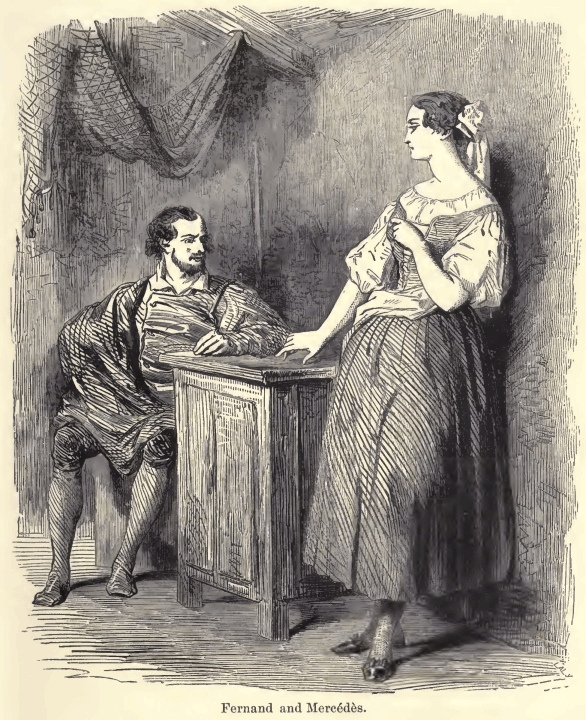
\includegraphics[width=\textwidth]{0045m.jpg}
\end{figure}

“You mistake, Fernand; it is not a law, but merely a custom, and, I
pray of you, do not cite this custom in your favor. You are included in
the conscription, Fernand, and are only at liberty on sufferance,
liable at any moment to be called upon to take up arms. Once a soldier,
what would you do with me, a poor orphan, forlorn, without fortune,
with nothing but a half-ruined hut and a few ragged nets, the miserable
inheritance left by my father to my mother, and by my mother to me? She
has been dead a year, and you know, Fernand, I have subsisted almost
entirely on public charity. Sometimes you pretend I am useful to you,
and that is an excuse to share with me the produce of your fishing, and
I accept it, Fernand, because you are the son of my father’s brother,
because we were brought up together, and still more because it would
give you so much pain if I refuse. But I feel very deeply that this
fish which I go and sell, and with the produce of which I buy the flax
I spin,—I feel very keenly, Fernand, that this is charity.”

“And if it were, Mercédès, poor and lone as you are, you suit me as
well as the daughter of the first shipowner or the richest banker of
Marseilles! What do such as we desire but a good wife and careful
housekeeper, and where can I look for these better than in you?”

“Fernand,” answered Mercédès, shaking her head, “a woman becomes a bad
manager, and who shall say she will remain an honest woman, when she
loves another man better than her husband? Rest content with my
friendship, for I say once more that is all I can promise, and I will
promise no more than I can bestow.”

“I understand,” replied Fernand, “you can endure your own wretchedness
patiently, but you are afraid to share mine. Well, Mercédès, beloved by
you, I would tempt fortune; you would bring me good luck, and I should
become rich. I could extend my occupation as a fisherman, might get a
place as clerk in a warehouse, and become in time a dealer myself.”

“You could do no such thing, Fernand; you are a soldier, and if you
remain at the Catalans it is because there is no war; so remain a
fisherman, and contented with my friendship, as I cannot give you
more.”

“Well, I will do better, Mercédès. I will be a sailor; instead of the
costume of our fathers, which you despise, I will wear a varnished hat,
a striped shirt, and a blue jacket, with an anchor on the buttons.
Would not that dress please you?”

“What do you mean?” asked Mercédès, with an angry glance,—“what do you
mean? I do not understand you?”

“I mean, Mercédès, that you are thus harsh and cruel with me, because
you are expecting someone who is thus attired; but perhaps he whom you
await is inconstant, or if he is not, the sea is so to him.”

“Fernand,” cried Mercédès, “I believed you were good-hearted, and I was
mistaken! Fernand, you are wicked to call to your aid jealousy and the
anger of God! Yes, I will not deny it, I do await, and I do love him of
whom you speak; and, if he does not return, instead of accusing him of
the inconstancy which you insinuate, I will tell you that he died
loving me and me only.” The young girl made a gesture of rage. “I
understand you, Fernand; you would be revenged on him because I do not
love you; you would cross your Catalan knife with his dirk. What end
would that answer? To lose you my friendship if he were conquered, and
see that friendship changed into hate if you were victor. Believe me,
to seek a quarrel with a man is a bad method of pleasing the woman who
loves that man. No, Fernand, you will not thus give way to evil
thoughts. Unable to have me for your wife, you will content yourself
with having me for your friend and sister; and besides,” she added, her
eyes troubled and moistened with tears, “wait, wait, Fernand; you said
just now that the sea was treacherous, and he has been gone four
months, and during these four months there have been some terrible
storms.”

Fernand made no reply, nor did he attempt to check the tears which
flowed down the cheeks of Mercédès, although for each of these tears he
would have shed his heart’s blood; but these tears flowed for another.
He arose, paced a while up and down the hut, and then, suddenly
stopping before Mercédès, with his eyes glowing and his hands
clenched,—“Say, Mercédès,” he said, “once for all, is this your final
determination?”

“I love Edmond Dantès,” the young girl calmly replied, “and none but
Edmond shall ever be my husband.”

“And you will always love him?”

“As long as I live.”

Fernand let fall his head like a defeated man, heaved a sigh that was
like a groan, and then suddenly looking her full in the face, with
clenched teeth and expanded nostrils, said,—“But if he is dead——”

“If he is dead, I shall die too.”

“If he has forgotten you——”

“Mercédès!” called a joyous voice from without,—“Mercédès!”

“Ah,” exclaimed the young girl, blushing with delight, and fairly
leaping in excess of love, “you see he has not forgotten me, for here
he is!” And rushing towards the door, she opened it, saying, “Here,
Edmond, here I am!”

Fernand, pale and trembling, drew back, like a traveller at the sight
of a serpent, and fell into a chair beside him. Edmond and Mercédès
were clasped in each other’s arms. The burning Marseilles sun, which
shot into the room through the open door, covered them with a flood of
light. At first they saw nothing around them. Their intense happiness
isolated them from all the rest of the world, and they only spoke in
broken words, which are the tokens of a joy so extreme that they seem
rather the expression of sorrow. Suddenly Edmond saw the gloomy, pale,
and threatening countenance of Fernand, as it was defined in the
shadow. By a movement for which he could scarcely account to himself,
the young Catalan placed his hand on the knife at his belt.

“Ah, your pardon,” said Dantès, frowning in his turn; “I did not
perceive that there were three of us.” Then, turning to Mercédès, he
inquired, “Who is this gentleman?”

“One who will be your best friend, Dantès, for he is my friend, my
cousin, my brother; it is Fernand—the man whom, after you, Edmond, I
love the best in the world. Do you not remember him?”

“Yes!” said Dantès, and without relinquishing Mercédès’ hand clasped in
one of his own, he extended the other to the Catalan with a cordial
air. But Fernand, instead of responding to this amiable gesture,
remained mute and trembling. Edmond then cast his eyes scrutinizingly
at the agitated and embarrassed Mercédès, and then again on the gloomy
and menacing Fernand. This look told him all, and his anger waxed hot.

“I did not know, when I came with such haste to you, that I was to meet
an enemy here.”

“An enemy!” cried Mercédès, with an angry look at her cousin. “An enemy
in my house, do you say, Edmond! If I believed that, I would place my
arm under yours and go with you to Marseilles, leaving the house to
return to it no more.”

Fernand’s eye darted lightning. “And should any misfortune occur to
you, dear Edmond,” she continued with the same calmness which proved to
Fernand that the young girl had read the very innermost depths of his
sinister thought, “if misfortune should occur to you, I would ascend
the highest point of the Cape de Morgiou and cast myself headlong from
it.”

Fernand became deadly pale. “But you are deceived, Edmond,” she
continued. “You have no enemy here—there is no one but Fernand, my
brother, who will grasp your hand as a devoted friend.”

And at these words the young girl fixed her imperious look on the
Catalan, who, as if fascinated by it, came slowly towards Edmond, and
offered him his hand. His hatred, like a powerless though furious wave,
was broken against the strong ascendancy which Mercédès exercised over
him. Scarcely, however, had he touched Edmond’s hand when he felt he
had done all he could do, and rushed hastily out of the house.

“Oh,” he exclaimed, running furiously and tearing his hair—“Oh, who
will deliver me from this man? Wretched—wretched that I am!”

“Hallo, Catalan! Hallo, Fernand! where are you running to?” exclaimed a
voice.

The young man stopped suddenly, looked around him, and perceived
Caderousse sitting at table with Danglars, under an arbor.

“Well”, said Caderousse, “why don’t you come? Are you really in such a
hurry that you have no time to pass the time of day with your friends?”

“Particularly when they have still a full bottle before them,” added
Danglars. Fernand looked at them both with a stupefied air, but did not
say a word.

“He seems besotted,” said Danglars, pushing Caderousse with his knee.
“Are we mistaken, and is Dantès triumphant in spite of all we have
believed?”

“Why, we must inquire into that,” was Caderousse’s reply; and turning
towards the young man, said, “Well, Catalan, can’t you make up your
mind?”

Fernand wiped away the perspiration steaming from his brow, and slowly
entered the arbor, whose shade seemed to restore somewhat of calmness
to his senses, and whose coolness somewhat of refreshment to his
exhausted body.

“Good-day,” said he. “You called me, didn’t you?” And he fell, rather
than sat down, on one of the seats which surrounded the table.

“I called you because you were running like a madman, and I was afraid
you would throw yourself into the sea,” said Caderousse, laughing.
“Why, when a man has friends, they are not only to offer him a glass of
wine, but, moreover, to prevent his swallowing three or four pints of
water unnecessarily!”

Fernand gave a groan, which resembled a sob, and dropped his head into
his hands, his elbows leaning on the table.

“Well, Fernand, I must say,” said Caderousse, beginning the
conversation, with that brutality of the common people in which
curiosity destroys all diplomacy, “you look uncommonly like a rejected
lover;” and he burst into a hoarse laugh.

“Bah!” said Danglars, “a lad of his make was not born to be unhappy in
love. You are laughing at him, Caderousse.”

“No,” he replied, “only hark how he sighs! Come, come, Fernand,” said
Caderousse, “hold up your head, and answer us. It’s not polite not to
reply to friends who ask news of your health.”

“My health is well enough,” said Fernand, clenching his hands without
raising his head.

“Ah, you see, Danglars,” said Caderousse, winking at his friend, “this
is how it is; Fernand, whom you see here, is a good and brave Catalan,
one of the best fishermen in Marseilles, and he is in love with a very
fine girl, named Mercédès; but it appears, unfortunately, that the fine
girl is in love with the mate of the \textit{Pharaon}; and as the \textit{Pharaon}
arrived today—why, you understand!”

“No; I do not understand,” said Danglars.

“Poor Fernand has been dismissed,” continued Caderousse.

“Well, and what then?” said Fernand, lifting up his head, and looking
at Caderousse like a man who looks for someone on whom to vent his
anger; “Mercédès is not accountable to any person, is she? Is she not
free to love whomsoever she will?”

“Oh, if you take it in that sense,” said Caderousse, “it is another
thing. But I thought you were a Catalan, and they told me the Catalans
were not men to allow themselves to be supplanted by a rival. It was
even told me that Fernand, especially, was terrible in his vengeance.”

Fernand smiled piteously. “A lover is never terrible,” he said.

“Poor fellow!” remarked Danglars, affecting to pity the young man from
the bottom of his heart. “Why, you see, he did not expect to see Dantès
return so suddenly—he thought he was dead, perhaps; or perchance
faithless! These things always come on us more severely when they come
suddenly.”

“Ah, \textit{ma foi}, under any circumstances!” said Caderousse, who drank as
he spoke, and on whom the fumes of the wine began to take
effect,—“under any circumstances Fernand is not the only person put out
by the fortunate arrival of Dantès; is he, Danglars?”

“No, you are right—and I should say that would bring him ill-luck.”

“Well, never mind,” answered Caderousse, pouring out a glass of wine
for Fernand, and filling his own for the eighth or ninth time, while
Danglars had merely sipped his. “Never mind—in the meantime he marries
Mercédès—the lovely Mercédès—at least he returns to do that.”

During this time Danglars fixed his piercing glance on the young man,
on whose heart Caderousse’s words fell like molten lead.

“And when is the wedding to be?” he asked.

“Oh, it is not yet fixed!” murmured Fernand.

“No, but it will be,” said Caderousse, “as surely as Dantès will be
captain of the \textit{Pharaon}—eh, Danglars?”

Danglars shuddered at this unexpected attack, and turned to Caderousse,
whose countenance he scrutinized, to try and detect whether the blow
was premeditated; but he read nothing but envy in a countenance already
rendered brutal and stupid by drunkenness.

“Well,” said he, filling the glasses, “let us drink to Captain Edmond
Dantès, husband of the beautiful Catalane!”

Caderousse raised his glass to his mouth with unsteady hand, and
swallowed the contents at a gulp. Fernand dashed his on the ground.

“Eh, eh, eh!” stammered Caderousse. “What do I see down there by the
wall, in the direction of the Catalans? Look, Fernand, your eyes are
better than mine. I believe I see double. You know wine is a deceiver;
but I should say it was two lovers walking side by side, and hand in
hand. Heaven forgive me, they do not know that we can see them, and
they are actually embracing!”

Danglars did not lose one pang that Fernand endured.

“Do you know them, Fernand?” he said.

“Yes,” was the reply, in a low voice. “It is Edmond and Mercédès!”

“Ah, see there, now!” said Caderousse; “and I did not recognize them!
Hallo, Dantès! hello, lovely damsel! Come this way, and let us know
when the wedding is to be, for Fernand here is so obstinate he will not
tell us.”

“Hold your tongue, will you?” said Danglars, pretending to restrain
Caderousse, who, with the tenacity of drunkards, leaned out of the
arbor. “Try to stand upright, and let the lovers make love without
interruption. See, look at Fernand, and follow his example; he is
well-behaved!”

\begin{figure}[h]
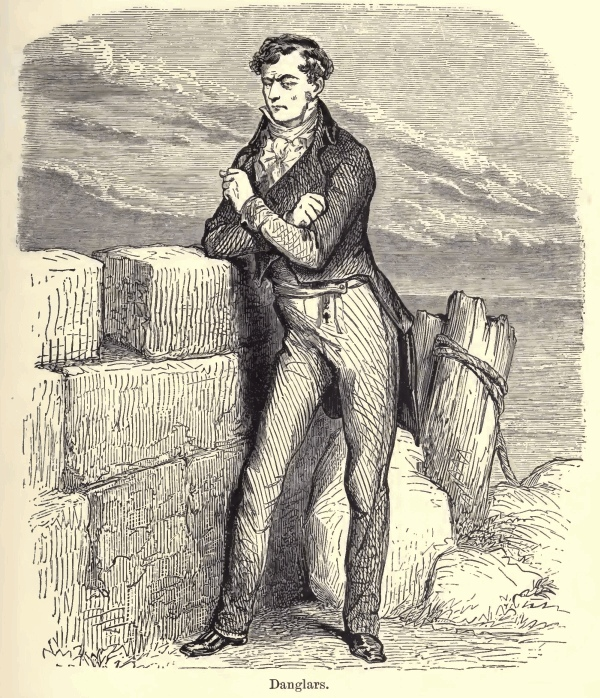
\includegraphics[width=\textwidth]{0051m.jpg}
\end{figure}

Fernand, probably excited beyond bearing, pricked by Danglars, as the
bull is by the bandilleros, was about to rush out; for he had risen
from his seat, and seemed to be collecting himself to dash headlong
upon his rival, when Mercédès, smiling and graceful, lifted up her
lovely head, and looked at them with her clear and bright eyes. At this
Fernand recollected her threat of dying if Edmond died, and dropped
again heavily on his seat. Danglars looked at the two men, one after
the other, the one brutalized by liquor, the other overwhelmed with
love.

“I shall get nothing from these fools,” he muttered; “and I am very
much afraid of being here between a drunkard and a coward. Here’s an
envious fellow making himself boozy on wine when he ought to be nursing
his wrath, and here is a fool who sees the woman he loves stolen from
under his nose and takes on like a big baby. Yet this Catalan has eyes
that glisten like those of the vengeful Spaniards, Sicilians, and
Calabrians, and the other has fists big enough to crush an ox at one
blow. Unquestionably, Edmond’s star is in the ascendant, and he will
marry the splendid girl—he will be captain, too, and laugh at us all,
unless”—a sinister smile passed over Danglars’ lips—“unless I take a
hand in the affair,” he added.

“Hallo!” continued Caderousse, half-rising, and with his fist on the
table, “hallo, Edmond! do you not see your friends, or are you too
proud to speak to them?”

“No, my dear fellow!” replied Dantès, “I am not proud, but I am happy,
and happiness blinds, I think, more than pride.”

“Ah, very well, that’s an explanation!” said Caderousse. “How do you
do, Madame Dantès?”

Mercédès courtesied gravely, and said—“That is not my name, and in my
country it bodes ill fortune, they say, to call a young girl by the
name of her betrothed before he becomes her husband. So call me
Mercédès, if you please.”

“We must excuse our worthy neighbor, Caderousse,” said Dantès, “he is
so easily mistaken.”

“So, then, the wedding is to take place immediately, M. Dantès,” said
Danglars, bowing to the young couple.

“As soon as possible, M. Danglars; today all preliminaries will be
arranged at my father’s, and tomorrow, or next day at latest, the
wedding festival here at La Réserve. My friends will be there, I hope;
that is to say, you are invited, M. Danglars, and you, Caderousse.”

“And Fernand,” said Caderousse with a chuckle; “Fernand, too, is
invited!”

“My wife’s brother is my brother,” said Edmond; “and we, Mercédès and
I, should be very sorry if he were absent at such a time.”

Fernand opened his mouth to reply, but his voice died on his lips, and
he could not utter a word.

“Today the preliminaries, tomorrow or next day the ceremony! You are in
a hurry, captain!”

“Danglars,” said Edmond, smiling, “I will say to you as Mercédès said
just now to Caderousse, ‘Do not give me a title which does not belong
to me’; that may bring me bad luck.”

“Your pardon,” replied Danglars, “I merely said you seemed in a hurry,
and we have lots of time; the \textit{Pharaon} cannot be under weigh again in
less than three months.”

“We are always in a hurry to be happy, M. Danglars; for when we have
suffered a long time, we have great difficulty in believing in good
fortune. But it is not selfishness alone that makes me thus in haste; I
must go to Paris.”

“Ah, really?—to Paris! and will it be the first time you have ever been
there, Dantès?”

“Yes.”

“Have you business there?”

“Not of my own; the last commission of poor Captain Leclere; you know
to what I allude, Danglars—it is sacred. Besides, I shall only take the
time to go and return.”

“Yes, yes, I understand,” said Danglars, and then in a low tone, he
added, “To Paris, no doubt to deliver the letter which the grand
marshal gave him. Ah, this letter gives me an idea—a capital idea! Ah;
Dantès, my friend, you are not yet registered number one on board the
good ship \textit{Pharaon};” then turning towards Edmond, who was walking
away, “A pleasant journey,” he cried.

“Thank you,” said Edmond with a friendly nod, and the two lovers
continued on their way, as calm and joyous as if they were the very
elect of heaven.
